% \chapter{Project Structure and Features}
\chapter{Cấu trúc dự án và các tính năng}
\label{ch:project_structure}

\section{Cấu trúc mã nguồn và mô hình ứng dụng}
\label{sec:source_code_structure}

Dự án Spotify Clone được xây dựng theo kiến trúc microservice, với mã nguồn được tổ chức trong thư mục gốc. Môi trường phát triển được thiết lập bằng Dev Containers và công cụ quản lý gói \texttt{uv}. File \texttt{serverclontify.sql} được sử dụng để mount vào PostgreSQL, đóng vai trò như một bản backup cơ sở dữ liệu. Thư mục \texttt{baseSetup} chứa các file mẫu để tạo nhanh các service mới.

\subsection{Cấu trúc thư mục gốc}
\label{subsec:root_directory_structure}

Cấu trúc thư mục gốc của dự án bao gồm:

\begin{verbatim}
./
+-- appServices/
|   +-- auth/
|   +-- common/
|   +-- music/
|   +-- storage/
|   +-- users/
+-- baseSetup/
+-- database/
+-- .devcontainer/
+-- example.env
+-- images/
+-- requirements.txt
+-- serverclontify.sql
+-- test/
+-- uv.lock
+-- pyproject.toml
\end{verbatim}

Trong đó:
\begin{itemize}
    \item \texttt{appServices/}: Chứa các microservice của ứng dụng.
    \item \texttt{baseSetup/}: Chứa các file cấu hình mẫu để tạo service mới.
    \item \texttt{database/}: Chứa các script liên quan đến cơ sở dữ liệu.
    \item \texttt{.devcontainer/}: Chứa cấu hình cho môi trường phát triển Dev Containers.
    \item \texttt{.env}: File cho các biến môi trường.
    \item \texttt{images/}: Chứa các hình ảnh sử dụng trong tài liệu hoặc ứng dụng.
    \item \texttt{requirements.txt}: Liệt kê các dependency chung của dự án.
    \item \texttt{serverclontify.sql}: File SQL backup cho cơ sở dữ liệu PostgreSQL.
    \item \texttt{test/}: Chứa các test case của dự án.
    \item \texttt{uv.lock}: File lock cho công cụ quản lý gói \texttt{uv}.
    \item \texttt{pyproject.toml}: File cấu hình cho các công cụ build và quản lý dự án Python.
\end{itemize}

\subsection{Cấu trúc một Microservice}
\label{subsec:microservice_structure}

Mỗi microservice trong thư mục \texttt{appServices} được xây dựng dựa trên framework Django và tuân theo mô hình MVC kết hợp pattern Controller/Service/Repository. Cấu trúc thư mục điển hình của một service (ví dụ: \texttt{auth}) như sau:

\begin{verbatim}
appServices/*/
+-- app/
|   +-- __init__.py
|   +-- controllers/
|   |   +-- ...
|   +-- entities/
|   |   +-- ...
|   +-- grpc/
|   |   +-- protos/
|   |       +-- *Service.proto
|   |       +-- *Service_pb2.py
|   |       +-- *Service_pb2_grpc.py
|   +-- migrations/
|   |   +-- ...
|   +-- models.py
|   +-- repositories/
|   |   +-- ...
|   +-- serializers/
|   |   +-- ...
|   +-- services/
|   |   +-- ...
|   +-- urls.py
+-- common/
+-- config/
|   +-- __init__.py
|   +-- asgi.py
|   +-- settings.py
|   +-- urls.py
|   +-- wsgi.py
+-- Dockerfile
+-- manage.py
+-- requirements.txt
\end{verbatim}

Trong đó, thư mục \texttt{app/} chứa các thành phần MVC và pattern C/S/R, thư mục \texttt{grpc/protos/} chứa các file định nghĩa gRPC và các file Python được build từ chúng.

File \texttt{Dockerfile} của mỗi service chịu trách nhiệm build image Docker cho service đó. Quá trình build bao gồm cài đặt các dependency từ \texttt{requirements.txt} và build các file Python từ các file \texttt{.proto}.

\subsection{Các Microservice hiện tại}
\label{subsec:existing_microservices}

Hiện tại, dự án bao gồm các microservice sau:

\begin{itemize}
    \item \textbf{auth service}: Quản lý việc đăng ký và đăng nhập người dùng, bao gồm 2 bảng \texttt{account} và \texttt{roles}. Khi đăng ký, service này gọi gRPC sang \texttt{users service} để tạo profile người dùng.
    \item \textbf{users service}: Quản lý thông tin người dùng thông qua bảng \texttt{profile}. Trong tương lai, service này sẽ có thêm bảng \texttt{favorite} để quản lý quan hệ nhiều-nhiều giữa người dùng và bài hát.
    \item \textbf{music service}: Quản lý thông tin về nhạc, thể loại và album với 6 bảng: \texttt{albums}, \texttt{albumSong}, \texttt{genres}, \texttt{genreSong}, \texttt{songs}, \texttt{songSubArtist}. Service này tương tác với \texttt{users service} qua gRPC để kiểm tra thông tin người dùng trước khi thêm nhạc hoặc sub-artist, và tương tác với \texttt{storage service} qua gRPC để lấy thông tin về phiên upload trên S3 (lưu ID phiên storage thay vì link trực tiếp).
    \item \textbf{storage service}: Quản lý các phiên upload thông qua bảng \texttt{storageData}.
    \item \textbf{common/}: Chứa các module hoặc code dùng chung giữa các service.
\end{itemize}

\section{Xây dựng Database cho Project}
\label{sec:database_design}

Dự án sử dụng PostgreSQL làm hệ quản trị cơ sở dữ liệu. Mỗi microservice quản lý các bảng dữ liệu riêng biệt để đảm bảo tính độc lập và phân tách mối quan tâm. Dưới đây là mô tả các bảng dữ liệu chính trong từng microservice:

\subsection{Database của auth service}
\label{subsec:db_auth_service}

\textbf{Bảng \texttt{accounts}:} Lưu trữ thông tin tài khoản người dùng.
\begin{itemize}
    \item \texttt{id} (UUID, primary key): ID duy nhất của tài khoản.
    \item \texttt{roleId} (UUID): ID của vai trò người dùng, tham chiếu đến bảng \texttt{roles}.
    \item \texttt{username} (VARCHAR(50), unique): Tên đăng nhập duy nhất của người dùng.
    \item \texttt{email} (EmailField, unique): Địa chỉ email duy nhất của người dùng.
    \item \texttt{password} (TEXT): Mật khẩu đã được hash của người dùng.
\end{itemize}
\textbf{Bảng \texttt{roles}:} Lưu trữ thông tin về các vai trò người dùng (ví dụ: admin, user).
\begin{itemize}
    \item \texttt{id} (UUID, primary key): ID duy nhất của vai trò.
    \item \texttt{name} (VARCHAR(50), unique): Tên duy nhất của vai trò.
    \item \texttt{description} (TEXT, nullable): Mô tả chi tiết về vai trò.
\end{itemize}

\subsection{Database của music service}
\label{subsec:db_music_service}

\textbf{Bảng \texttt{albums}:} Lưu trữ thông tin về các album nhạc.
\begin{itemize}
    \item \texttt{id} (UUID, primary key): ID duy nhất của album.
    \item \texttt{name} (VARCHAR(255)): Tên của album.
    \item \texttt{description} (TEXT, nullable): Mô tả chi tiết về album.
    \item \texttt{storageImageId} (UUID, nullable): ID tham chiếu đến ảnh bìa của album trong bảng \texttt{storageData} của \texttt{storage service}.
    \item \texttt{artistId} (UUID): ID của nghệ sĩ tạo album.
\end{itemize}
\textbf{Bảng \texttt{albumSong}:} Bảng trung gian thể hiện mối quan hệ nhiều-nhiều giữa album và bài hát.
\begin{itemize}
    \item \texttt{albumId} (UUID): ID của album, tham chiếu đến bảng \texttt{albums}.
    \item \texttt{songId} (UUID): ID của bài hát, tham chiếu đến bảng \texttt{songs}.
    \item \texttt{order} (PositiveIntegerField, nullable): Thứ tự của bài hát trong album.
\end{itemize}
\textbf{Bảng \texttt{genres}:} Lưu trữ thông tin về các thể loại nhạc.
\begin{itemize}
    \item \texttt{id} (UUID, primary key): ID duy nhất của thể loại.
    \item \texttt{name} (VARCHAR(100), unique): Tên duy nhất của thể loại.
    \item \texttt{description} (TEXT, nullable): Mô tả chi tiết về thể loại.
\end{itemize}
\textbf{Bảng \texttt{genreSong}:} Bảng trung gian thể hiện mối quan hệ nhiều-nhiều giữa thể loại và bài hát.
\begin{itemize}
    \item \texttt{songID} (UUID): ID của bài hát, tham chiếu đến bảng \texttt{songs}.
    \item \texttt{genreID} (UUID): ID của thể loại, tham chiếu đến bảng \texttt{genres}.
\end{itemize}
\textbf{Bảng \texttt{songs}:} Lưu trữ thông tin về các bài hát.
\begin{itemize}
    \item \texttt{id} (UUID, primary key): ID duy nhất của bài hát.
    \item \texttt{title} (VARCHAR(255)): Tiêu đề của bài hát.
    \item \texttt{description} (VARCHAR, nullable): Mô tả ngắn về bài hát.
    \item \texttt{artistId} (UUID): ID của nghệ sĩ thể hiện bài hát.
    \item \texttt{storageId} (UUID, unique): ID tham chiếu đến file âm thanh của bài hát trong bảng \texttt{storageData} của \texttt{storage service}.
    \item \texttt{storageImageId} (UUID, nullable): ID tham chiếu đến ảnh bìa của bài hát trong bảng \texttt{storageData} của \texttt{storage service}.
    \item \texttt{duration} (PositiveIntegerField, nullable): Thời lượng của bài hát (tính bằng giây).
    \item \texttt{songType} (VARCHAR(255)): Loại bài hát (ví dụ: audio, video).
\end{itemize}
\textbf{Bảng \texttt{songSubArtist}:} Bảng trung gian thể hiện mối quan hệ nhiều-nhiều giữa bài hát và các nghệ sĩ phụ (sub-artist).
\begin{itemize}
    \item \texttt{songID} (UUID): ID của bài hát, tham chiếu đến bảng \texttt{songs}.
    \item \texttt{subArtistID} (UUID): ID của nghệ sĩ phụ.
\end{itemize}

\subsection{Database của storage service}
\label{subsec:db_storage_service}

\textbf{Bảng \texttt{storageData}:} Lưu trữ thông tin về các file đã upload.
\begin{itemize}
    \item \texttt{id} (UUID, primary key): ID duy nhất của bản ghi storage.
    \item \texttt{userId} (UUID): ID của người dùng đã tải file lên.
    \item \texttt{fileName} (VARCHAR(255), unique): Tên file gốc.
    \item \texttt{fileType} (VARCHAR(255)): Loại file (ví dụ: audio/mpeg, video/mp4, image/jpeg).
    \item \texttt{fileSize} (IntegerField): Kích thước file (tính bằng byte).
    \item \texttt{fileUrl} (URLField, nullable): URL truy cập đến file trên S3.
    \item \texttt{description} (TEXT, nullable): Mô tả về file.
\end{itemize}

\subsection{Database của users service}
\label{subsec:db_users_service}

\textbf{Bảng \texttt{profiles}:} Lưu trữ thông tin hồ sơ người dùng.
\begin{itemize}
    \item \texttt{id} (UUID, primary key): ID duy nhất của profile.
    \item \texttt{accountID} (UUID, unique): ID tham chiếu đến tài khoản người dùng trong bảng \texttt{accounts} của \texttt{auth service}.
    \item \texttt{fullName} (TEXT(150)): Tên đầy đủ của người dùng.
    \item \texttt{avatarUrl} (URLField, nullable): URL đến ảnh đại diện của người dùng.
    \item \texttt{bio} (TEXT(500), nullable): Tiểu sử ngắn của người dùng.
    \item \texttt{dateOfBirth} (DateField, nullable): Ngày sinh của người dùng.
    \item \texttt{phoneNumber} (CharField(20), nullable): Số điện thoại của người dùng.
\end{itemize}
\begin{comment}
\textbf{Bảng \texttt{favorite} (sẽ được thêm):} Bảng trung gian thể hiện mối quan hệ nhiều-nhiều giữa người dùng và bài hát yêu thích.
\begin{itemize}
    \item \texttt{userId} (UUID): ID của người dùng.
    \item \texttt{songId} (UUID): ID của bài hát.
    \item \texttt{timestamp} (DateTimeField): Thời điểm thêm vào danh sách yêu thích.
    \item \textit{(Có thể có thêm các trường khác)}
\end{itemize}
\end{comment}


\section{Các tính năng được xây dựng}
\label{sec:built_features}

Dưới đây là danh sách các tính năng cơ bản đã được xây dựng trong dự án:

\subsection{Chức năng đăng nhập}
\label{subsec:dang-nhap}

Chức năng đăng nhập cho phép người dùng truy cập vào hệ thống bằng tài khoản cá nhân. Người dùng cần nhập đúng tên đăng nhập và mật khẩu đã đăng ký trước đó. Hệ thống sẽ xác thực thông tin và chuyển hướng người dùng đến trang chính nếu thành công.

\begin{figure}
    \centering
    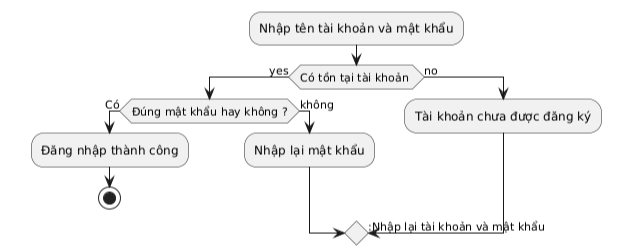
\includegraphics[width=1\linewidth]{images/flowchart-dang-nhap.png}
    \caption{Flowchart chức năng đăng nhập}
    \label{fig:flowchart-dang-nhap}
\end{figure}

\subsection{Chức năng đăng ký}
\label{subsec:dang-ky}

Chức năng đăng ký cho phép người dùng tạo tài khoản mới để sử dụng hệ thống. Người dùng cần cung cấp thông tin như tên đăng nhập, mật khẩu và các thông tin cá nhân cần thiết. Sau khi đăng ký thành công, người dùng có thể sử dụng tài khoản để đăng nhập và trải nghiệm dịch vụ.

\begin{figure}
    \centering
    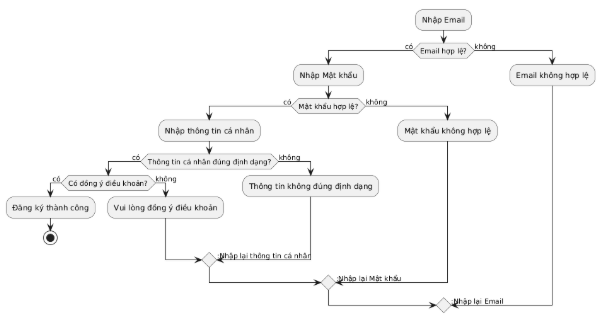
\includegraphics[width=1\linewidth]{images/flowchart-dang-ky.png}
    \caption{Flowchart chức năng đăng ký}
    \label{fig:flowchart-dang-ky}
\end{figure}

\subsection{Chức năng quên mật khẩu}
\label{subsec:quen-mat-khau}

Chức năng quên mật khẩu cho phép người dùng khôi phục mật khẩu bằng cách nhập email đã đăng ký và nhận liên kết hoặc mã xác thực để thiết lập mật khẩu mới, đảm bảo bảo mật tài khoản và hỗ trợ truy cập lại hệ thống một cách nhanh chóng.

\begin{figure}
    \centering
    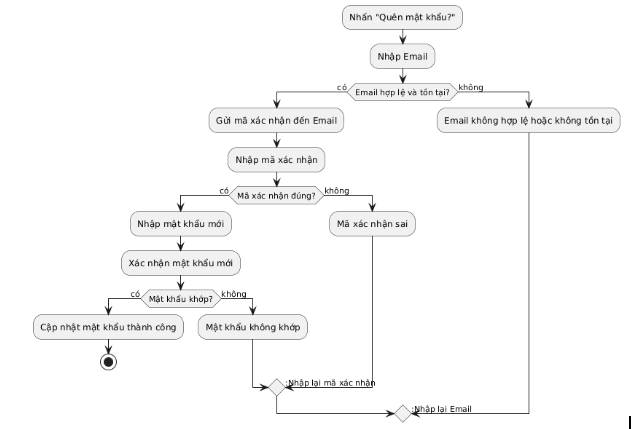
\includegraphics[width=1\linewidth]{images/flowchart-quen-mat-khau.png}
    \caption{Flowchart chức năng quên mật khẩu}
    \label{fig:flowchart-quen-mat-khau}
\end{figure}

\subsection{Màn hình trang chủ}
\label{subsec:trang-chu}

Trang chủ hiển thị danh sách nhạc nổi bật, playlist cá nhân hóa và các đề xuất dựa trên thói quen nghe nhạc của người dùng, giúp trải nghiệm âm nhạc trở nên phong phú, trực quan và sinh động như giao diện của Spotify.

\begin{figure}
    \centering
    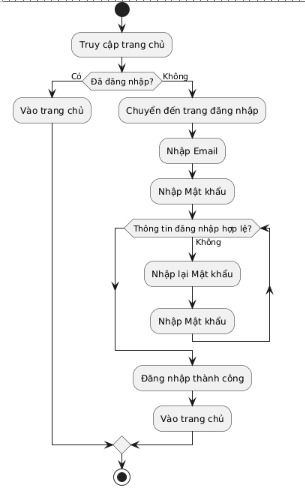
\includegraphics[width=1\linewidth]{images/flowchart-trang-chu.png}
    \caption{Flowchart màn hình trang chủ}
    \label{fig:flowchart-trang-chu}
\end{figure}

\subsection{Màn hình hồ sơ}
\label{subsec:ho-so}

Trang hồ sơ cá nhân hiển thị ảnh đại diện, tên người dùng và thay đổi mật khẩu giúp người dùng quản lý thông tin của mình dễ hơn.

\begin{figure}
    \centering
    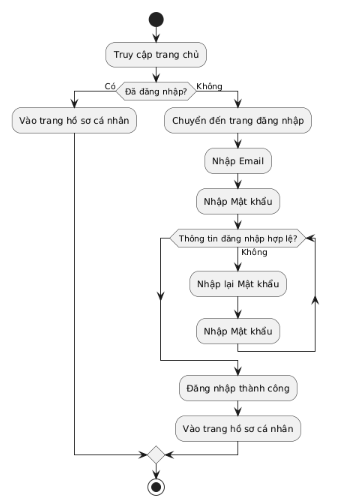
\includegraphics[width=1\linewidth]{images/flowchart-ho-so.png}
    \caption{Flowchart hồ sơ}
    \label{fig:flowchart-ho-so}
\end{figure}

\subsection{Màn hình nghệ sĩ}
\label{subsec:nghe-si}

Trang nghệ sĩ hiển thị ảnh đại diện, tiểu sử, số người theo dõi, danh sách album, bài hát nổi bật và các sự kiện liên quan, giúp người dùng khám phá âm nhạc.

\begin{figure}
    \centering
    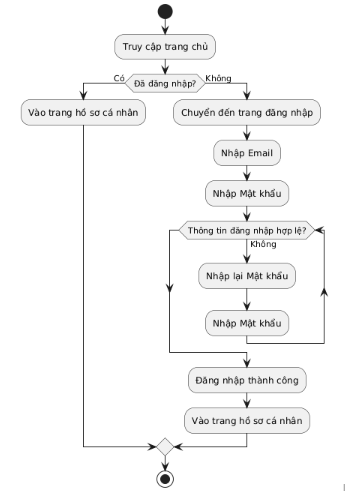
\includegraphics[width=1\linewidth]{flowchart-nghe-si.png}
    \caption{Flowchart màn hình nghệ sĩ}
    \label{fig:flowchart-nghe-si}
\end{figure}

\subsection{Màn hình Album}
\label{subsec:album}

Trang album hiển thị ảnh bìa, tên album, tên nghệ sĩ, ngày phát hành và danh sách bài hát trong album, cho phép người dùng nghe từng bài hoặc phát toàn bộ, mang đến trải nghiệm nghe nhạc trọn vẹn và trực quan như trên Spotify.


\begin{figure}
    \centering
    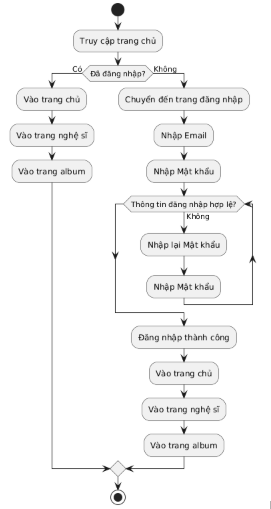
\includegraphics[width=0.8\linewidth]{images/flowchart-album.png}
    \caption{Flowchart màn hình album}
    \label{fig:flowchart-album}
\end{figure}

\subsection{Chức năng tìm kiếm}
\label{subsec:tim-kiem}

Trang tìm kiếm nhạc cho phép người dùng nhập từ khóa để tìm bài hát, nghệ sĩ, album, đồng thời hiển thị kết quả theo từng danh mục rõ ràng, giúp việc khám phá âm nhạc trở nên nhanh chóng và tiện lợi như trên Spotify.

\begin{figure}
    \centering
    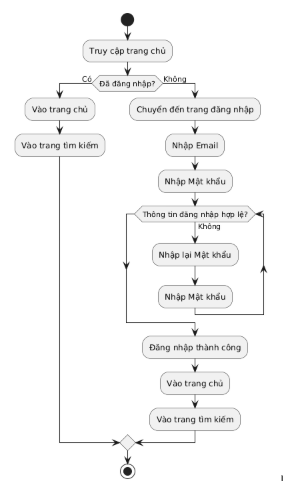
\includegraphics[width=1\linewidth]{images/flowchart-tim-kiem.png}
    \caption{Flowchart tìm kiếm}
    \label{fig:flowchart-tim-kiem}
\end{figure}

\subsection{Màn hình bài hát yêu thích}
\label{subsec:yeu-thich}

Chức năng tạo playlist cho phép người dùng tạo danh sách phát riêng, chọn tên, sau đó thêm nhạc từ các bài hát yêu thích hoặc tìm kiếm, giúp cá nhân hóa trải nghiệm nghe nhạc giống như trên Spotify.

\begin{figure}
    \centering
    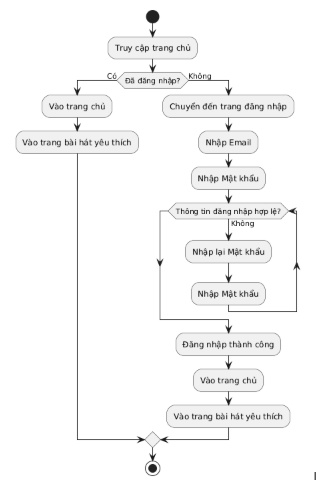
\includegraphics[width=1\linewidth]{images/flowchart-yeu-thich.png}
    \caption{Flowchart màn hình bài hát yêu thích}
    \label{fig:flowchart-yeu-thich}
\end{figure}

\subsection{Admin}
\label{subsec:admin}

\begin{figure}
    \centering
    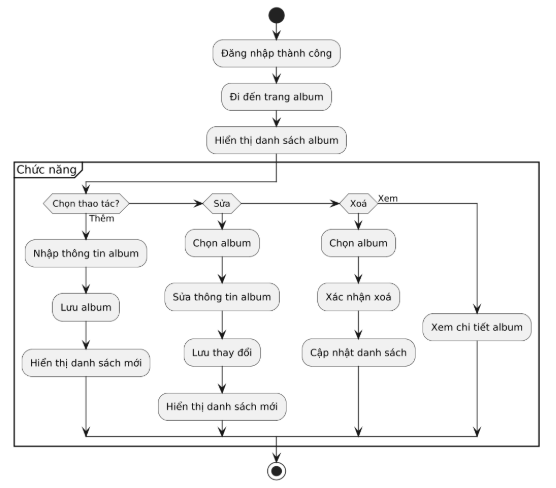
\includegraphics[width=1\linewidth]{images/flowchart-admin-album.png}
    \caption{Flowchart chức năng quản lý Album của Admin}
    \label{fig:flowchart-admin-album}
\end{figure}

\begin{figure}
    \centering
    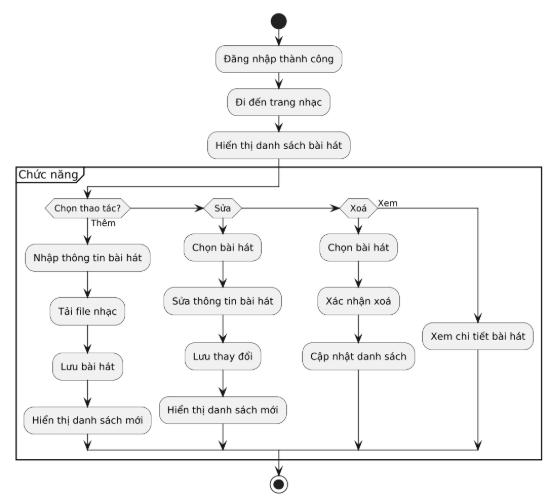
\includegraphics[width=1\linewidth]{images/flowchart-admin-music.png}
    \caption{Flowchart chức năng quản lý Music của Admin}
    \label{fig:flowchart-admin-music}
\end{figure}

\begin{figure}
    \centering
    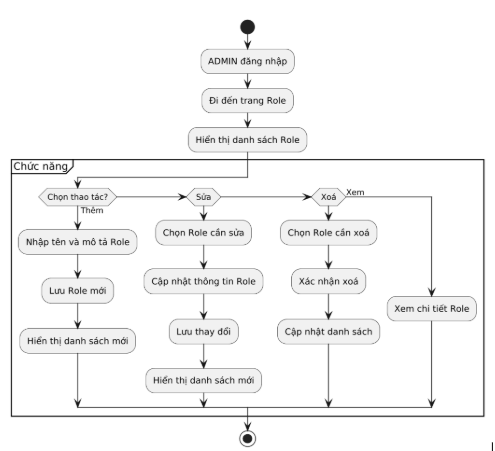
\includegraphics[width=1\linewidth]{images/flowchart-admin-role.png}
    \caption{Flowchart chức năng quản lý Role của Admin}
    \label{fig:flowchart-admin-role}
\end{figure}

\begin{figure}
    \centering
    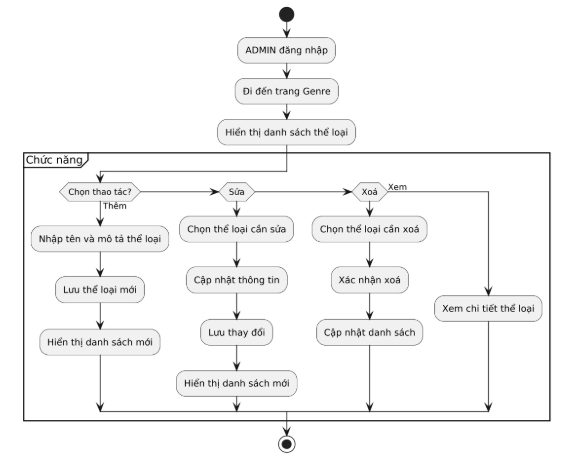
\includegraphics[width=1\linewidth]{images/flowchart-admin-genre.png}
    \caption{Flowchart chức năng quản lý Genre của Admin}
    \label{fig:flowchart-admin-genre}
\end{figure}

\begin{figure}
    \centering
    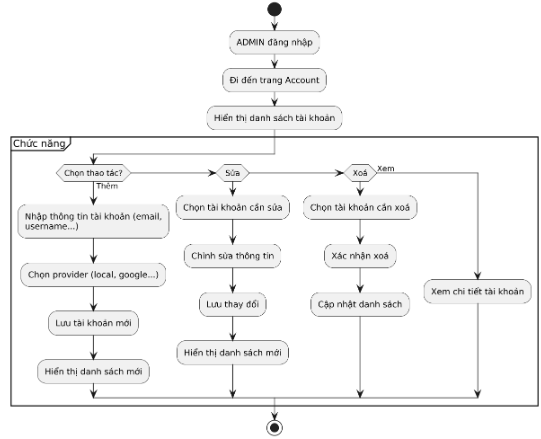
\includegraphics[width=1\linewidth]{images/flowchart-admin-account.png}
    \caption{Flowchart chức năng quản lý Account của Admin}
    \label{fig:flowchart-admin-account}
\end{figure}